% (C) 2020 Diogo Rodrigues
% Licensed under Creative Commons Attribution-NonCommercial-NoDerivatives 4.0 International (CC-BY-NC-ND 4.0)

\documentclass{sope}
\usepackage[english]{babel}
% Metadata
\title{SOPE -- Exam 2016/17}
\author{Diogo Miguel Ferreira Rodrigues \\ \email{dmfrodrigues2000@gmail.com}}
% Document
\begin{document}

\setcounter{chapter}{16}
\exam{Exam 2016/17}
\question{Question 1}
\begin{tabular}{p{29mm} | p{122mm}}
    DMA & Allows some hardware subsystems (usually peripherals) to directly access certain principal memory regions. This means the CPU is only required to start or end transactions, and the actual transactions can be performed by the subsystems, freeing CPU time. \\ \hline
    Test\&Set instruction & Hardware instruction that can be used to implement mutual exclusion and mutexes. Sets variable to 1 and returns the previous value atomically, so a critical section can be implemented by first calling Test\&Set for the \emph{mutex} until it returns 0, execute the section and then set the \emph{mutex} to 0. \\ \hline
    Valid/invalid page bit & Essential part of a virtual memory implementation. There is a table that has a valid/invalid bit for each page, which is set to 1 if it is currently loaded in principal memory, so this bit allows to know if a page is loaded in memory (i.e., can access it) or not (i.e., needs to load that page and only then can it be accessed).
\end{tabular}

\question{Question 2}
\begin{lstlisting}[language=C]
// Global
init(ready1, 0);
init(ready2, 0);
init(ready3, 0);
\end{lstlisting}
\begin{tabular}{p{49mm} p{49mm} p{49mm}}
    \begin{lstlisting}[language=C]
// P1
sinal(ready1);
wait(ready2);
signal(ready2);
wait(ready3);
signal(ready3);
// A    
    \end{lstlisting} &
    \begin{lstlisting}[language=C]
// P2
sinal(ready2);
wait(ready1);
signal(ready1);
wait(ready3);
signal(ready3);
// B    
    \end{lstlisting} &
    \begin{lstlisting}[language=C]
// P3
sinal(ready3);
wait(ready1);
signal(ready1);
wait(ready2);
signal(ready2);    
// C
    \end{lstlisting}
\end{tabular}

\questionitem{Item b}
This solution does not cause deadlocks, since the \emph{hold and wait} condition is false. This is because none of the three processes tries to lock more resources while holding the lock for other resources. This is obvious because, immediately after waiting for a semaphore, a process immediately signals that same semaphore in the following statement. This is allowed because the problem statement mentions process 1 must wait for 2 and 3 to reach B and C respecively but is not required to hold the locks during execution of block A, so it basically only needs to be notified that processes 2 and 3 reached B and C. Initially semaphores are set to 0, so when process 2 reaches B it signals \texttt{ready2}. Once process 1 waits for \texttt{ready2}, when that call returns process 1 is considered to have been successfully notified that process 2 has reached block B, so it does not have to keep \texttt{ready2} locked.

\question{Question 3}
Processor scheduling refers to the scheduling of which processes will be executed and by what order, so as to optimize a certain set or criteria.

Preemptive scheduling algorithms can force a process to stop, even if the process has not blocked or yielded the CPU, to free CPU time for other processes.

A CPU-bound process is a process whose execution time is mostly bounded by CPU performance, and that usually has a few very long CPU bursts. This is usually contrasted to I/O-bound processes which are mostly bounded by I/O operations performance, and that usually have lots of very short CPU bursts.

The statement that preemptive processor scheduling favours CPU-bound processes is false, since we can present the preemptive Shortest Job First algorithm as a counter-example. This algorithm forcibly assigns the CPU to the active process that has the least estimated future CPU burst duration $T_n$, even if that implies forcibly stopping an already running process to yield the CPU to a process that arrived afterwards. By the definition of I/O-bound processes, these have very low CPU burst durations so $T_n$ will be small. This means a CPU-bound process can be starved if several I/O-bound processes are also active, since the I/O-bound processes will almost always have precedence over CPU-bound processes due to lower $T_n$. So this is an example of a preemptive scheduling algorithm that does not favour CPU-bound processes, making the question statement false.

\question{Question 4}
\questionitem{Item a}
\textbf{(1)} The address refers to page 2, offset 125

To find the page we just need to get the result of the integer division between the address and the page size $\SI{512}{\byte}=2^9\SI{}{\byte}$; or otherwise just right-shift by 9.

\begin{equation*}
    0000010001111101_2 / 2^9 = 0000010001111101_2 >> 9 = 0000010_2 = 2
\end{equation*}

It was loaded to page 2.

The offset can be found by getting the integer division remainder between the address and the page size; or otherwise just take the first 9 bits.

\begin{equation*}
    0000010001111101_2~\%~2^9 = 0000010001111101_2~\&~111111111_2 = 001111101_2 = 64+32+16+8+4+1 = 125 
\end{equation*}

\textbf{(2)} In a page-based memory management system, pages and frames have the same size, so the frame size is $2^9\SI{}{\byte}$. To find the physical address, we have to add the page factor $2^9 \cdot page$ and the offset factor $offset$. When a page is mapped to a frame, each byte in a page at a certain offset from page beginning is mapped to the byte at the same offset of frame beginning, so $offset=125$.

The address is thus $2^9 \cdot 15 + 125 = (1111_2 << 9)~|~001111101_2 = 1111000000000_2~|~001111101_2 = 0001111001111101_2 $

\questionitem{Item b}
\textbf{(1)} Thrashing is when a process spends more time performing pagination activities than otherwise actually executing. This can be detected by evaluating the faults/access ratio, which should be close to 0 for normal operation and close to 1 for a very serious thrashing situation.

\textbf{(2)} Thrashing can be stopped through various ways, some of which include swapping out some processes, or requiring pages to stay in principal or secondary memory for at least a certain minimum duration.

\textbf{(3)} Yes it is possible to avoid thrashing, namely by using strategies like:
\begin{itemize}
    \item Working-Set strategy: try to predict the number of frames and what pages to keep for a process based on recent process needs.
    \item Page-Fault Rate strategy: define a range of acceptable page-fault rates and assign/remove a frame from a process according to its page-fault rate.
\end{itemize}

\question{Question 5}
\questionitem{Item a}
Append mode should be used so the processes' output do not overwrite. If \texttt{O\_APPEND} was not used, each process would keep a different file cursor, and a process P1 write would start at P1 cursor, but if another process P2 had already written in the area following P1 cursor then P1 would start writting in its own cursor position and overwrite the data written by P2. By using \texttt{O\_APPEND}, a write call first seeks the end of file and only then does it write to the file.

\questionitem{Item b}
If append mode was not available, we could use a strategy similar to that which append mode implements: seek end of file and write. We could otherwise use a synchronized cursor for all processes, by allocating it in shared memory (protected by a mutex to avoid race conditions over the cursor). There is a chance there would also be a need to create a mutex to avoid race conditions over the file itself (for append mode mutual exclusivity is guaranteed, but not necessarily if append mode is not used).

\question{Question 6}
\questionitem{Item a}
\begin{lstlisting}[language=C]
    int numbits = atoi(argv[1]);
\end{lstlisting}
\begin{lstlisting}[language=C]
    execl("/home/sope/gen_bit", "/home/sope/gen_bit", NULL);
\end{lstlisting}
Place this in line 16:
\begin{lstlisting}[language=C]
    printf("%.*s\n", numbits, bits);
\end{lstlisting}

\questionitem{Item b}
\texttt{gen\_bit} provides as \emph{random} result the last bit of its PID, or otherwise its parity. Since the generated \texttt{gen\_bit} processes have consecutive PIDs the result of any \texttt{gen\_seq} run will have alternating 0's and 1's, since consecutive PID's mean alternated PID parities. So for a sequence of length $N$ there are really only two possible results: alternated 0's and 1's starting in 0, or starting in 1.

\questionitem{Item c}
One could then shuffle \texttt{bits} right after line 15, using the statement
\begin{lstlisting}[language=C]
    shuffle(bits, numbits);
\end{lstlisting}
where \texttt{void shuffle(char *v, int n)} shuffles array \texttt{v} of size \texttt{n} using the pseudo-random number generator \texttt{rand()}.

Randomness would still be limited because there would still only be $2\binom{N}{\lfloor N/2 \rfloor}$ (all sequences of $N$ bits, with $\lfloor N/2 \rfloor$ 0's or $\lfloor N/2 \rfloor$ 1's), when there could be $2^N$ possibilities.

\questionitem{Item d}
Remove line 13; make \texttt{bits} global and declare it before line 1; between lines 2 and 3 add
\begin{lstlisting}[language=C]
    signal(SIGUSR1, signal_handler);
    signal(SIGUSR2, signal_handler);
\end{lstlisting}
and before line 2 add the definition of \texttt{signal\_handler}:
\begin{lstlisting}[language=C]
void signal_handler(int sig){
    if     (sig == SIGUSR1) strcat(bits, "0");
    else if(sig == SIGUSR2) strcat(bits, "1");
}
\end{lstlisting}

\question{Question 7}
\questionitem{Item a}
I would use two named FIFOs for each pair of communicating threads. I would additionally use a message queue so process 1 could inform process 2 that it has a thread that wants to communicate with process 2.
\begin{center}
    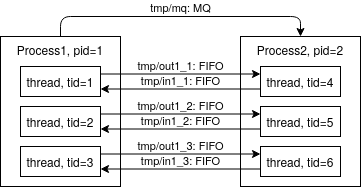
\includegraphics[scale=0.5]{2017N_07_a}
\end{center}

\questionitem{Item b}
To communicate, \texttt{Process1} executes
\begin{lstlisting}[language=C,basicstyle=\ttfamily\small]
pid_t pid = getpid();
pthread_t tid = pthread_self();
// Create FIFOs
char out_name[256];
if(sprintf(out_name,"/tmp/out%d_%d",pid,tid)<0){perror("sprintf out");exit(1);}
char in_name [256];
if(sprintf(in_name ,"/tmp/in%d_%d" ,pid,tid)<0){perror("sprintf in" );exit(1);}
if(mkfifo(out_name, 0777))                     {perror("mkfifo out" );exit(1);}
int out_fd = open(out_name, O_WRONLY);
if(out_fd < 0)                                 {perror("open out"   );exit(1);}
if(mkfifo(in_name , 0777))                     {perror("mkfifo in"  );exit(1);}
int in_fd = open(in_name, O_RDONLY);
if(in_fd < 0)                                  {perror("open in"    );exit(1);}
\end{lstlisting}
Now the current thread can communicate with process 2 using \texttt{out\_fd} and \texttt{in\_fd}.

\questionitem{Item c}
The queue is created by \texttt{Process2} using
\begin{lstlisting}[language=C,basicstyle=\ttfamily\small]
mqd_t mq = mq_open("/tmp/mq", O_CREAT | O_RDONLY, 0777, NULL);
if(mq == 1) exit(1);
\end{lstlisting}
\texttt{Process1} announces it wants to communicate by sending:
\begin{lstlisting}[language=C,basicstyle=\ttfamily\small]
typedef struct {
    pid_t pid,
    pthread_t tid;
} Message;
// Send message through message queue
mqd_t mq = mq_open("/tmp/mq", O_WRONLY);
if(mq == 1)                                    {perror("mq_open mq" );exit(1);}
Message message = {
    .pid = getpid(),
    .tid = pthread_self()
};
if(mq_send(mq, &message, sizeof(Message), 0))  {perror("mq_send tid");exit(1);}
if(mq_close(mq))                               {perror("mq_close mq");exit(1);}
\end{lstlisting}

\questionitem{Item d}
If a call to \texttt{open} a FIFO with flags \texttt{O\_WRONLY|O\_NONBLOCK} fails with \texttt{errno=ENXIO}, that means there is no process with the FIFO open for reading, so a thread can close its write-only FIFO and try to open it again to check if the read end is still open (i.e., if the other thread is still alive).

In the case of a thread in \texttt{Process1}, it would evaluate:
\begin{lstlisting}[language=C,basicstyle=\ttfamily\small]
if(close(out_fd))   {perror("close out_fd");exit(1);}
int out_fd = open(out_name, O_WRONLY|O_NONBLOCK);
if(out_fd < 0){
    if(errno == ENXIO){
        // The other thread stopped working
    } else          {perror("open out"   );exit(1);}
}
\end{lstlisting}

\questionitem{Item e}
\begin{lstlisting}[language=C,basicstyle=\ttfamily\small]
if(close(out_fd))  { perror("close out"  ); exit(1); }
if(close(in_fd ))  { perror("close in"   ); exit(1); }
if(unlink(out_name){ perror("unlink out" ); exit(1); }
if(unlink(in_name ){ perror("unlink in"  ); exit(1); }
// Process1 on ending
if(mq_close(mq))   { perror("mq_close mq"); exit(1); }
\end{lstlisting}

\question{Question 8}
\questionitem{Item a}
\newpage
\begin{lstlisting}[language=C,basicstyle=\ttfamily\small]
// NRECEIVERS: global constant indicating the number of receivers; has value 10
pthread_t receivers_tid[NRECEIVERS], caller_tid;
for(int i = 0; i < NRECEIVERS; ++i){
    int *index = malloc(sizeof(int));
    *index = i+1;
    pthread_create(&receivers_tid[i], NULL, receiver, index);
}
pthread_create(&caller_tid, NULL, caller, NULL);
\end{lstlisting}

\questionitem{Item b}
To make sure the number of received calls is correctly counted, I would use a mutex to protect \texttt{numPhoneCalls} from simultaneous access by several threads. To do this, I would probably make the \texttt{while} loop infinite and break once \texttt{numPhoneCalls >= MAX\_NUM\_PHONE\_CALLS}, since this would make it easier to correctly lock and unlock the mutex.

To inform \texttt{caller} that he has to make a call, we could declare a global variable \texttt{winnerNumber} and a semaphore starting with value 0, and on receiving a winner call a receiver would, on line 9, set \texttt{winnerNumber} to the winner phone number and also signal that semaphore. The \texttt{caller} would be on a cycle, calling \texttt{wait} on that semaphore. Once it unblocks the caller knows \texttt{winnerNumber} contains a number that he should call.

\questionitem{Item c}
\begin{lstlisting}[language=C,basicstyle=\ttfamily\small]
// At the beginning, as Global
pthread_mutex_t mutex = PTHREAD_MUTEX_INITIALIZER;
int winnerNumber;
sem_t sem;
// In main
int main(){
    sem_init(&sem, 0);
    ...
    return 0;
}
\end{lstlisting}

\questionitem{Item d}
\begin{lstlisting}[language=C,basicstyle=\ttfamily\small]
// MAX_NUM_PHONE_CALLS: constante global que indica o no max. total de chamadas
while (true) {
    pthread_mutex_lock(&mutex);
    if(numPhoneCalls >= MAX_NUM_PHONE_CALLS) break;
    pthread_mutex_unlock(&mutex);
    // espera ate que chegue uma chamada telefonica e "anota" o numero de telefone
    int phoneNumber = receiveCall();
    pthread_mutex_lock(&mutex);
    int numCalls = ++numPhoneCalls;
    pthread_mutex_unlock(&mutex);
    if (numCalls % 1000 == 0) {
        // o concorrente cujo numero de telefone e phoneNumber e um dos vencedores
        // informa o thread caller que deve fazer uma chamada para phoneNumber
        winnerNumber = phoneNumber;
        sem_signal(&sem);
    }
}
\end{lstlisting}

\end{document}